\subsection{Diagrama de bloques}

La solución propuesta consta de tres entidades, aunque dos pueden ser el mismo dispositivo: \begin{itemize}
    \item Sistema de carga y monitorización de baterías. Compuesto por la electrónica diseñada (\autoref{subsec:montaje_completo}) y la inteligencia del ESP8266. 
    \item Servidor de medidas. Compuesto por un \textit{Broker MQTT} al que enviar las medidas y un \textit{Dashboard} en la que representarlas. En nuestro caso, se trata de una máquina virtual Ubuntu en la que se instala \textit{Thingsboard}, un software que cumple ambas funciones. (\autoref{subsec:thingsboard})
    \item Cliente web. Cualquier dispositivo con un navegador web puede acceder al \textit{Dashboard} para visualizar la información.
\end{itemize}

Se puede ver el diagrama de bloques en la \autoref{fig:diagrama_bloques_general}

\begin{figure}[H]
    \centering
    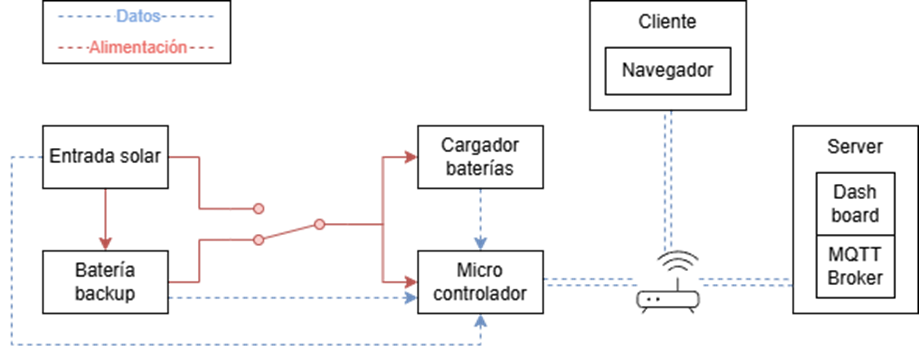
\includegraphics[width=0.8\textwidth]{images/2-hardware/bloquesGeneral.png}
    \caption{Diagrama de bloques general de la solución}
    \label{fig:diagrama_bloques_general}
\end{figure}
